\documentclass[12pt,a4paper]{report}
\usepackage[top=1in, bottom=1in, left=1in, right=1in]{geometry}
\usepackage{graphicx}
\usepackage{svg}
\usepackage{tikz}
\usetikzlibrary{calc} 
\usepackage{tabularx}
\usepackage{amsmath, amsfonts, amssymb, amsthm}
\usepackage{graphicx}
\usepackage{cite}
\usepackage[final]{hyperref}
\usepackage{cite}
\usepackage{algorithm}
\usepackage{algpseudocode}
\usepackage{tikz}

\usepackage{listings, booktabs, caption}
\usepackage{listings, color}
\usepackage{fancyhdr}
\fancyhead[L]{CE244 LAB3}
\usepackage{setspace}
\onehalfspacing
\usepackage[T1]{fontenc}
\usepackage{xcolor}
\usepackage{listings, xcolor,svg}
\usepackage{listings}
\usepackage{color}
\usepackage{graphicx, caption}



\definecolor{Green}{rgb}{0,0.6,0}
\definecolor{Gray}{rgb}{0.5,0.5,0.5}
\definecolor{Mauve}{rgb}{0.58,0,0.82}
\definecolor{Purple}{HTML}{800080}
\definecolor{Mulberry}{rgb}{0.77, 0.29, 0.55}
\definecolor{WildStrawberry}{rgb}{1.0, 0.26, 0.64}


\definecolor{coolblack}{rgb}{0.0, 0.18, 0.39}
\definecolor{oxfordblue}{rgb}{0.0, 0.13, 0.28}
\definecolor{prussianblue}{rgb}{0.0, 0.19, 0.33}
\definecolor{bostonuniversityred}{rgb}{0.8, 0.0, 0.0}
\hypersetup{
	colorlinks=true,
	linkcolor=bostonuniversityred,
	citecolor=blue,
	filecolor=magenta,
	urlcolor=blue         
}
\usepackage{pdfpages}
\usepackage{listings}
\usepackage{xcolor}
\usepackage{caption}
\usepackage{float}

\definecolor{keywordcolor}{rgb}{0.5,0,0.5}
\definecolor{stringcolor}{rgb}{0.6,0.6,0}
\definecolor{commentcolor}{rgb}{0.0,0.5,0.0}
\definecolor{backgroundcolor}{rgb}{1.0,1.0,1.0}
\definecolor{numbercolor}{rgb}{0.5,0.5,0.5}

\lstset{
    backgroundcolor=\color{backgroundcolor},
    basicstyle=\ttfamily\normalsize, % Set font size here
    breakatwhitespace=false,
    breaklines=true,
    captionpos=b,
    commentstyle=\color{commentcolor}\itshape,
    extendedchars=true,
    frame=tb, % Draw lines above and below the code
    rulecolor=\color{black},
    framerule=0.5pt, % Line thickness
    framextopmargin=1pt,
    framexbottommargin=1pt,
    framesep=0pt,
    keepspaces=true,
    keywordstyle=\color{keywordcolor}\bfseries,
    language=Python,
    numbers=left,
    numbersep=10pt,
    numberstyle=\normalsize\color{numbercolor}, % Set line numbering font size
    showspaces=false,
    showstringspaces=false,
    showtabs=false,
    stepnumber=1,
    stringstyle=\color{stringcolor},
    tabsize=4,
    aboveskip=10pt, % Space above the code
    belowskip=10pt, % Space below the code
    belowcaptionskip=0pt
}
 % You need the soul package to use \hl
\newcommand{\hl}[1]{\texttt{#1}}
\usepackage[utf8]{inputenc}
\usepackage{amsmath}
\usepackage{amsfonts}
\usepackage{amssymb}
\usepackage{graphicx}
\usepackage{tikz}
\usepackage{fancyhdr}
\usepackage{lastpage}
\usetikzlibrary{shapes.geometric, arrows, positioning}

\tikzstyle{startstop} = [rectangle, rounded corners, minimum width=3cm, minimum height=1cm,text centered, draw=black, fill=red!30]
\tikzstyle{process} = [rectangle, minimum width=3cm, minimum height=1cm, text centered, draw=black, fill=orange!30]
\tikzstyle{decision} = [diamond, minimum width=3cm, minimum height=1cm, text centered, draw=black, fill=green!30]
\tikzstyle{arrow} = [thick,->,>=stealth]

\title{Voronoi Diagram}
\author{adzetto}
\date{\today}

\pagestyle{fancy}
\fancyhf{} % Clear all header and footer fields
\fancyhead[R]{Page \thepage\ of \pageref{LastPage}} % Page number in the upper right corner
\fancyhead[L]{CS106, Term Project, Spring 2024}
\fancyfoot[L]{İzmir Institute of Technology} % University name in the bottom left corner
\fancyfoot[R]{Mechanical Engineering Department} % Department name in the bottom right corner

\renewcommand{\footrulewidth}{0.1pt} % Define the width of the footer rule
\begin{document}

\maketitle

\begin{abstract}
    This project's goal is to use a collection of uniformly distributed points on a plane to construct the Voronoi cell that corresponds to a point at the origin. Making points, finding distances, finding the Voronoi cell, and then visualising the data are all part of this process. Our research shows how to do this in Python and identifies its strengths and weaknesses as a practical tool.

    \vfill
    An animation package called Manim was used to produce a simulation that would further show how the Voronoi diagram was generated. You can see the process of building the Voronoi cell for a point at the origin in this simulation. The following link will take you to YouTube, where you can see the simulation: \url{https://youtu.be/6qEfmROZ5AA}, \url{https://youtu.be/hTJOVJYhSf8}, \url{https://youtu.be/4JLaDXvqGDo}.
    \vfill
    Note. Code formatting is in accordance with \texttt{PEP 8 - Style Guide for Python Code}; \url{https://peps.python.org/pep-0008/} requirements. Guidelines for Python code organisation were drafted by Guido van Rossum, Barry Warsaw, and Alyssa Coghlan and are outlined in these guidelines. Following the guidelines laid down by \textit{PEP 8,} the code is now structured in this format.
\end{abstract}

\tableofcontents

\chapter{Introduction}

\section{Purpose}
The main goal of this project is to make the Voronoi cell that goes with a point at the origin in a plane that is filled with randomly placed points. The project includes several important steps: picking random points, figuring out how far these points are from the starting point, deciding where the edges of the Voronoi cell will be, and finally, showing the Voronoi cell on a graph. The study aims to give a full picture of the geometric features of Voronoi graphs and how they can be used in real life.


\section{Motivation}
There are many uses for voronoi diagrams in many fields, such as computer science, biology, and geography. They are an important part of computational geometry. The need to understand the academic and practical sides of these geometric shapes is what led to this project. In the area of computer science, Voronoi maps are used in images, location analysis, and methods for finding the shortest path. In geography, they are used to make maps and plan spaces, and in biology, they can be used to make models of cell structures and regions. By using a Voronoi model, this project aims to help people understand these uses better and lay the groundwork for more study and development.

\section{Aim}
The project's goal is to create a Python programme that can randomly place points in a plane, find the Voronoi cell that corresponds to a point at the origin, and draw that cell. To correctly calculate and see the Voronoi cell, this requires using a number of different computer methods and programmes.

\section{Objectives}
To achieve the aim of this project, the following specific objectives have been established:
\begin{itemize}
  \item To generate a set of randomly distributed points within a two-dimensional plane.
  \item To compute the distances from each of these points to a fixed point at the origin.
  \item To determine the boundaries of the Voronoi cell associated with the origin based on the calculated distances.
  \item To visualize the Voronoi cell along with the randomly generated points using appropriate plotting techniques.
\end{itemize}

\section{Scope}
Python and its tools, such as numpy and matplotlib, will be used in this project to make Voronoi diagrams and show them. Using this method, random points are made in polar coordinates, then they are changed to Cartesian coordinates and the Voronoi cell for the origin is calculated. For a better understanding of the Voronoi cell's structure, the results of this application will be shown in image form. This project is mostly about making a simple solution for a fixed point at the origin, but the methods and results can be used in more complicated situations with bigger datasets and different point distributions, which means the study can be used in more areas.


\section{Significance}
For many useful situations, it is important to know how Voronoi models are put together and what their features are. This project not only helps students learn how to understand geometric shapes, but it also lays the groundwork for more advanced uses in science and business. The study's findings can be used to make the best use of space resources, make computer programmes run faster, and create better models of nature events. These findings will greatly assist progress in both the theory and applied sciences.

\section{Structure of the Report}
The report is organized as follows:
\begin{itemize}
  \item \textbf{Chapter 2: Literature Review} - Summarises what has already been written about Voronoi diagrams, including their theory bases and real-world uses. It has parts about the past of Voronoi diagrams and other works in the same field.
  \item \textbf{Chapter 3: Proposed System Analysis \& Design} - Gives more information about the problem description, analysis, viability study, requirement analysis, and system design. Included in this chapter is a diagram that shows the steps that were taken to create and display the Voronoi cell.
  \item \textbf{Chapter 4: Technology Implementation \& Testing} - It talks about the technologies and tools that were used in the project, like Random, Numpy, Matplotlib, and Python. It includes the Python code and gives a thorough explanation of how to make a Voronoi map.
  \item \textbf{Chapter 5: Application, Advantages \& Limitations} - Talks about the different ways Voronoi diagrams can be used, the benefits of using them in different areas, and the problems with the way they are currently implemented.
  
  \item \textbf{Chapter 6: Conclusion and Future Work} - Summarises the project's results, talks about what those results mean, and offers possible areas for more study and changes in the future.
\end{itemize}


\chapter{Literature Review}

\section{Background History}

An essential building block of computational geometry, voronoi diagrams divide a plane into separate areas according to their distance from a predetermined set of points called generators. So, let \( P = \{p_1, p_2, \ldots, p_n\} \subset \mathbb{R}^2 \) be a set of \( n \) distinct points. The Voronoi cell \( V(p_i) \) associated with the generator \( p_i \in P \) is defined as:
\[
V(p_i) = \{ x \in \mathbb{R}^2 \mid \forall j \neq i, \|x - p_i\| \leq \|x - p_j\| \}
\]
where \( \|\cdot\| \) denotes the Euclidean norm. These regions, or cells, have broad applicability across multiple disciplines.

\section{Related Works}

Theoretical developments and practical uses of voronoi diagrams are covered extensively in the literature. Some notable innovations include iterative methods for building centroidal Voronoi tessellations (CVTs) and algorithms for efficient calculation of Voronoi diagrams (e.g., Fortune's sweepline algorithm). Let \( \Omega \subseteq \mathbb{R}^2 \) be a domain, and let \( \rho: \Omega \to \mathbb{R} \) be a density function. The objective in constructing a CVT is to find a set of points \( P \subset \Omega \) such that each point \( p_i \in P \) is the centroid of its respective Voronoi cell \( V(p_i) \), weighted by \( \rho \). Formally, \( p_i \) must satisfy:
\[
p_i = \frac{\int_{V(p_i)} x \rho(x) \, dx}{\int_{V(p_i)} \rho(x) \, dx}
\]
Geometric models are useful in many fields; for example, spatial analysis may help with location optimisation issues, and the biological sciences can use them to better understand cellular structures and patterns.

\section{Summary \& Discussion}

Voronoi diagrams and their centroidal variations are fundamentally important for studying their computational characteristics and applications. This knowledge makes it easier to create effective algorithms and put them into practice in a variety of real-world contexts.

\chapter{Proposed System Analysis \& Design}

\section{Problem Statement}

Given a point located at the origin \( O \in \mathbb{R}^2 \) and a set of randomly distributed points \( P = \{p_1, p_2, \ldots, p_n\} \subset \mathbb{R}^2 \), the task is to determine the Voronoi cell associated with the origin. Formally, we seek to compute the region:
\[
V(O) = \{ x \in \mathbb{R}^2 \mid \forall p_i \in P, \|x - O\| \leq \|x - p_i\| \}
\]
This involves generating points, calculating distances, and employing algebraic methods to delineate \( V(O) \).

\section{Analysis}

Python is used to create the points and calculate the required distances. The process of analysis is as follows: first, in polar coordinates, create \( P \). Then, transform it to Cartesian coordinates. Finally, calculate the distances in Euclidean terms from each point in \( P \) to the origin. How is the distance function defined:

\[
d_i = \|p_i - O\| = \sqrt{x_i^2 + y_i^2}
\]
for each \( p_i = (x_i, y_i) \in P \). The Voronoi cell \( V(O) \) is constructed by finding the perpendicular bisectors of the line segments \( [O, p_i] \) and determining their intersections.

\section{Feasibility Study}

\textbf{Technical Feasibility}: No specialised hardware or software is required since the project uses ordinary Python libraries like as \texttt{numpy}, \texttt{matplotlib}, and \texttt{random}.

\textbf{Economic Feasibility}: The cost is minimal, requiring only a computer with Python installed.

\textbf{Behavioral Feasibility}: The project is straightforward and accessible, making it suitable for educational and research purposes.

\section{Requirement Analysis}

The necessary tools include:
\begin{itemize}
  \item \texttt{Python}: For implementation.
  \item \texttt{numpy}: For numerical computations.
  \item \texttt{matplotlib}: For plotting results.
  \item \texttt{random}: For generating random points.
\end{itemize}

\section{System Design}

The design involves the following steps:

\begin{itemize}

\item[1 |]  Generate random points \( P \) in polar coordinates and convert to Cartesian coordinates.
\item[2 |] Compute distances \( d_i = \|p_i - O\| \) for each \( p_i \in P \).
\item[3 |] Identify the closest points to the origin and calculate the perpendicular bisectors of the segments \( [O, p_i] \).
\item[4 |] Determine the intersection points of these bisectors to form the boundaries of \( V(O) \).
\item[5 |] Plot the points and the Voronoi cell using \texttt{matplotlib}.
\end{itemize}


Mathematically, the perpendicular bisector of \( [O, p_i] \) can be described as:
\[
\text{Bisector}(O, p_i): (x - \frac{x_i}{2}) x_i + (y - \frac{y_i}{2}) y_i = 0
\]
Solving the system of linear equations given by the bisectors will yield the vertices of the Voronoi cell.


\subsection{Flowchart}

For now, I will just leave this here with a simple flowchar showing the process. I will give more details in the Implementation part.

\begin{figure}[ht!]
    \centering
    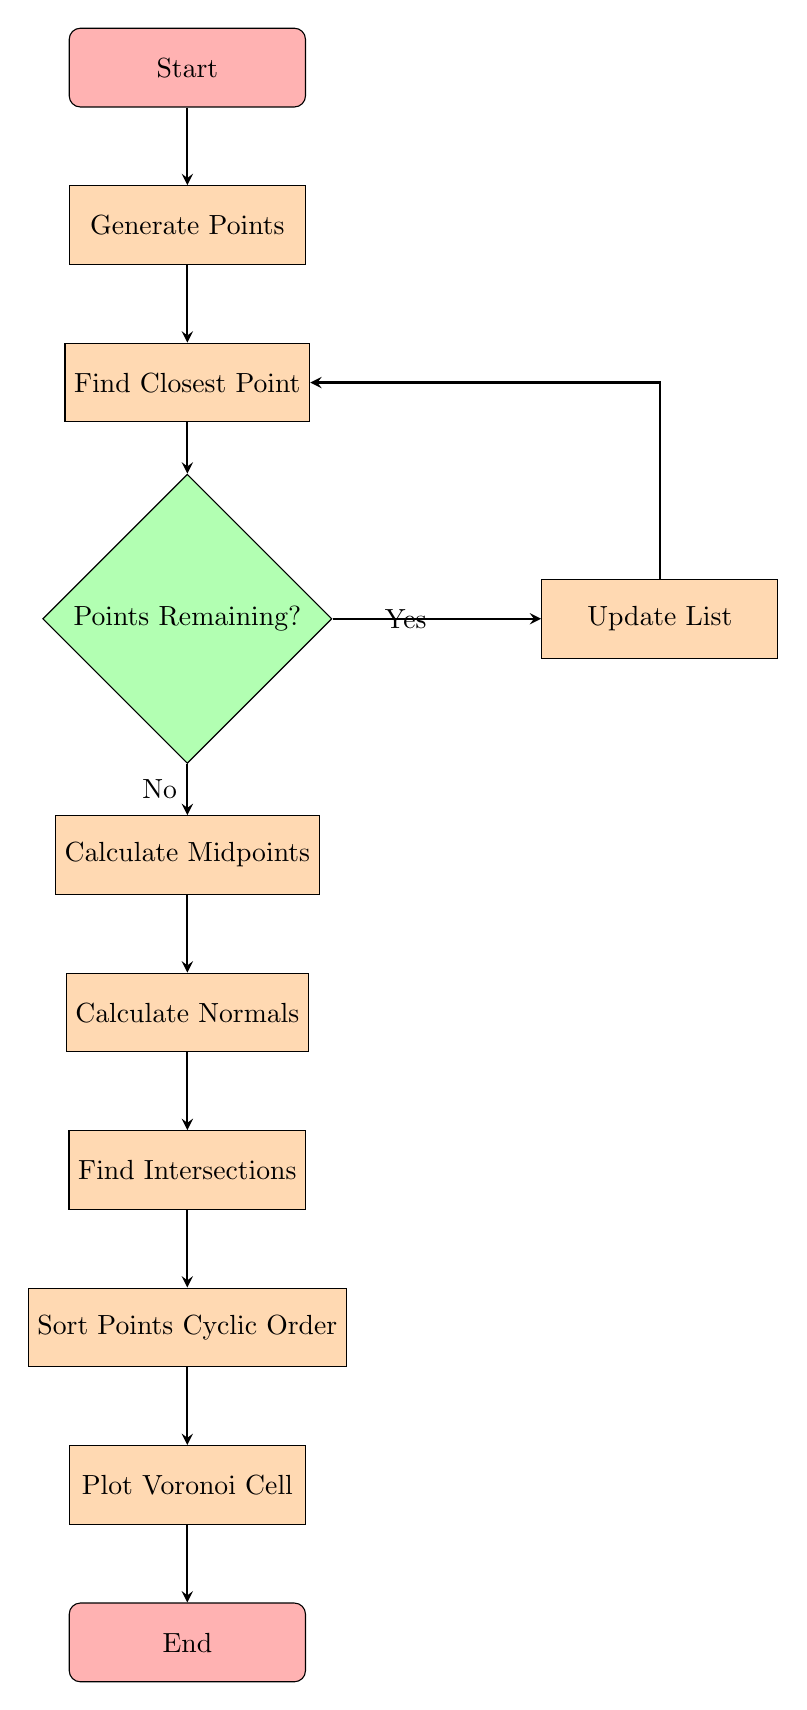
\begin{tikzpicture}[node distance=2cm]

        \node (start) [startstop] {Start};
        \node (generate) [process, below of=start] {Generate Points};
        \node (findClosest) [process, below of=generate] {Find Closest Point};
        \node (checkPoints) [decision, below of=findClosest, yshift=-1cm] {Points Remaining?};
        \node (updateList) [process, right of=checkPoints, xshift=4cm] {Update List};
        \node (midpoints) [process, below of=checkPoints, yshift=-1cm] {Calculate Midpoints};
        \node (normals) [process, below of=midpoints] {Calculate Normals};
        \node (intersect) [process, below of=normals] {Find Intersections};
        \node (sort) [process, below of=intersect] {Sort Points Cyclic Order};
        \node (plot) [process, below of=sort] {Plot Voronoi Cell};
        \node (end) [startstop, below of=plot] {End};

        \draw [arrow] (start) -- (generate);
        \draw [arrow] (generate) -- (findClosest);
        \draw [arrow] (findClosest) -- (checkPoints);
        \draw [arrow] (checkPoints) -- node[anchor=east] {Yes} (updateList);
        \draw [arrow] (updateList) |- (findClosest);
        \draw [arrow] (checkPoints) -- node[anchor=east] {No} (midpoints);
        \draw [arrow] (midpoints) -- (normals);
        \draw [arrow] (normals) -- (intersect);
        \draw [arrow] (intersect) -- (sort);
        \draw [arrow] (sort) -- (plot);
        \draw [arrow] (plot) -- (end);

    \end{tikzpicture}
    \caption{Flowchart of the Voronoi Diagram Generation Process}
\end{figure}

\chapter{Technology Implementation \& Testing}
\section{Technology}
\begin{itemize}
  \item \textbf{Python}: A high-level programming language used for implementing the project.
  \item \textbf{Numpy}: A library for numerical operations in Python.
  \item \textbf{Matplotlib}: A library for plotting graphs in Python.
  \item \textbf{Random}: A module for generating random numbers in Python.
\end{itemize}




\section{Implementation}

\subsection{Point Generation Function}

\subsubsection{Purpose}
The \texttt{generate\_points} function generates a specified number of points within given ranges for the radial and angular coordinates. These points are evenly distributed around the center and are transformed from polar to Cartesian coordinates.

\subsubsection{Arguments \& Returns}
Amount of points to create, denoted as $n$. $r_{min}$ is the smallest radius. the greatest radius, denoted as $r_{max}$. $\theta_{min}$: The angle with the smallest value (of degrees). In degrees, $\theta_{max}$ represents the greatest angle. This function takes an array of tuples as input and returns a new array with the distance from the origin as well as the x and y coordinates of each set.


\vspace*{\fill} \newpage

\subsubsection{Algorithm}

\begin{algorithm}
\caption{Generate Random Points in Polar Coordinates}
\begin{algorithmic}[1]
\Function{generate\_points}{$n, r_{min}, r_{max}, \theta_{min}, \theta_{max}$}
    \State $\mathcal{P} \gets \varnothing$
    \For{$i \gets 1$ to $n$}
        \State $r \gets \text{random.uniform}(r_{min}, r_{max})$
        \State $\theta \gets \text{random.uniform}(\theta_{min}, \theta_{max})$
        \State $x \gets r \cdot \cos(\theta)$
        \State $y \gets r \cdot \sin(\theta)$
        \State $d \gets \sqrt{x^2 + y^2}$
        \State $\mathcal{P} \gets \mathcal{P} \cup \{(x, y, d)\}$
    \EndFor
    \State \Return $\mathcal{P}$
\EndFunction
\end{algorithmic}
\end{algorithm}



\subsubsection{Explanation}
The function converts polar coordinates \((r, \theta)\) to Cartesian coordinates \((x, y)\) using:
\[
x = r \cdot \cos(\theta)
\]
\[
y = r \cdot \sin(\theta)
\]
The distance $d$ from the origin is calculated as:
\[
d = \sqrt{x^2 + y^2}
\]


\vspace*{\fill}\newpage

\subsubsection{Python Code}
\begin{figure}[ht!]
\centering
\caption*{\large\textit{points.py}}
\begin{lstlisting}[language=Python, caption={Function to Generate Points}]
import random
import math

def generate_points(n, r_min, r_max, theta_min, theta_max):
    points = []
    for _ in range(n):
        r = random.uniform(r_min, r_max)
        theta = random.uniform(theta_min, theta_max)
        x = r * math.cos(math.radians(theta))
        y = r * math.sin(math.radians(theta))
        distance = math.sqrt(x**2 + y**2)
        points.append((x, y, distance))
    return points
\end{lstlisting}
\end{figure}


\subsection{Generating Points in Different Angular Segments}

\subsubsection{Purpose}
To generate points inside defined angular segments in such a way that they are evenly distributed around the origin.


\subsubsection{Python Code}
\begin{figure}[ht!]
\centering
\caption*{\large\textit{main.py}}
\begin{lstlisting}[language=Python, caption={Generating Points in Different Angular Segments}]
points_first = (
    generate_points(n=5, r_min=2.5, r_max=15, theta_min=5, theta_max=85) +
    generate_points(n=5, r_min=2.5, r_max=15, theta_min=95, theta_max=175) +
    generate_points(n=5, r_min=2.5, r_max=15, theta_min=185, theta_max=265) +
    generate_points(n=5, r_min=2.5, r_max=15, theta_min=275, theta_max=355)
)
\end{lstlisting}
\end{figure}

\subsection{Finding the Closest Point Function}

\subsubsection{Purpose}
By removing previously found closest points, the \texttt{find\_closest\_point} function finds the point in a list of points that is closest to a reference point \( P_0 \).

\subsubsection{Arguments \& Returns}
The set of points is denoted by $\mathcal{P}$. Point $P_0$ is the starting point. In earlier rounds, the locations that were determined to be closest were added to the $\mathcal{C}$ list. Finds the point nearest to \( P_0 \) and returns its index and coordinates.

\subsubsection{Algorithm}

\begin{algorithm}
\caption{Find the Closest Point}
\begin{algorithmic}[1]
\Function{find\_closest\_point}{$\mathcal{P}, P_0, \mathcal{C}$}
    \State $\mathcal{P}_{\text{array}} \gets \text{array}([\mathbf{p}[:2] \ \text{for} \ \mathbf{p} \in \mathcal{P}])$
    \State $P_{0,\text{array}} \gets \text{array}(P_0)$
    \State $\mathcal{D} \gets \text{array}([\|\mathbf{p} - P_{0,\text{array}}\| \ \text{for} \ \mathbf{p} \in \mathcal{P}_{\text{array}}])$
    \For{$\mathbf{c} \in \mathcal{C}$}
        \If{$\mathbf{c} \in \mathcal{P}$}
            \State $index \gets \text{index}(\mathbf{c})$
            \State $\mathcal{D}[index] \gets \infty$
        \EndIf
    \EndFor
    \State $i_{\text{min}} \gets \text{argmin}(\mathcal{D})$
    \State \Return $(i_{\text{min}}, \mathcal{P}[i_{\text{min}}])$
\EndFunction
\end{algorithmic}
\end{algorithm}

\subsubsection{Explanation}

Consider the set of points \( \mathbf{p}_i = (x_i, y_i, d_i) \) where each point \( \mathcal{P} \subset \mathbb{R}^2 \times \mathbb{R} \) contains the coordinates and distance from the origin. In prior rounds, the set of points that were determined to be closest was denoted as \( \mathcal{C} \subset \mathcal{P} \) and the reference point was denoted as \( P_0 = (x_0, y_0) \in \mathbb{R}^2 \). Finding the point in \( \mathcal{P} \setminus \mathcal{C} \) that is closest to \( P_0 \) is the goal. The collection of coordinates of points in \( \mathcal{P} \) is defined as the array \( \mathcal{P}_{\text{array}} \).

\[
\mathcal{P}_{\text{array}} = \left\{ \mathbf{p}[:2] \mid \mathbf{p} \in \mathcal{P} \right\}
\]

Let \( P_{0,\text{array}} \) be the array representation of the reference point \( P_0 \):
\[
P_{0,\text{array}} = \text{array}(P_0)
\]

Compute the Euclidean distances \( \mathcal{D} \) from \( P_0 \) to each point in \( \mathcal{P}_{\text{array}} \):
\[
\mathcal{D} = \left\{ \|\mathbf{p} - P_{0,\text{array}}\| \mid \mathbf{p} \in \mathcal{P}_{\text{array}} \right\}
\]

For each point \( \mathbf{c} \in \mathcal{C} \), if \( \mathbf{c} \in \mathcal{P} \), set the corresponding distance in \( \mathcal{D} \) to \( \infty \) to exclude it from consideration:
\[
\text{For each } \mathbf{c} \in \mathcal{C}, \text{ if } \mathbf{c} \in \mathcal{P}, \text{ set } \mathcal{D}[\text{index}(\mathbf{c})] = \infty
\]

Determine the index \( i_{\text{min}} \) of the minimum distance in \( \mathcal{D} \):
\[
i_{\text{min}} = \text{argmin}(\mathcal{D})
\]

Return the index and coordinates of the closest point:
\[
\text{Return } (i_{\text{min}}, \mathcal{P}[i_{\text{min}}])
\]


After selecting all points and setting their distances to infinity, the function finds the one with the smallest Euclidean distance to \( P_0 \) and returns it.

\subsubsection{Python Code}
\begin{figure}[H]
\centering
\caption*{\large\textit{find\_closest.py}}
\begin{lstlisting}[language=Python, caption={Function to Find Closest Point}]
import numpy as np
from numpy.linalg import norm

def find_closest_point(points, P_0, closest_points):
    points_array = np.array([point[:2] for point in points])
    P_0_array = np.array(P_0)

    distances = np.array([norm(point - P_0_array) for point in points_array])
    for point in closest_points:
        if point in points:
            index = points.index(point)
            distances[index] = float('inf')

    closest_point_index = np.argmin(distances)
    return closest_point_index, points[closest_point_index]
\end{lstlisting}
\end{figure}

\subsection{Unit Vector Calculation Function}

\subsubsection{Purpose}
Geometric algorithms that need direction and normalisation rely on the \texttt{find\_unit\_vector} function, which computes the unit vector from one point to another.

\subsubsection{Arguments \& Return}
$P_{\text{from}}$: The starting point. $P_{\text{to}}$: The ending point. Returns the unit vector from $P_{\text{from}}$ to $P_{\text{to}}$.


\subsubsection{Algorithm}
\begin{algorithm}
\caption{Find Unit Vector}
\begin{algorithmic}[1]
\State \textbf{Input:} Points \( P_{\text{from}} = (x_{\text{from}}, y_{\text{from}}) \) and \( P_{\text{to}} = (x_{\text{to}}, y_{\text{to}}) \)
\State \textbf{Output:} Unit vector \( \hat{\mathbf{v}} \)

\State \( \mathbf{v} \gets \begin{pmatrix} x_{\text{to}} - x_{\text{from}} \\ y_{\text{to}} - y_{\text{from}} \end{pmatrix} \)
\Comment{Compute the difference vector}

\State \( \|\mathbf{v}\| \gets \sqrt{(x_{\text{to}} - x_{\text{from}})^2 + (y_{\text{to}} - y_{\text{from}})^2} \)
\Comment{Calculate the Euclidean norm of \(\mathbf{v}\)}

\If{\( \|\mathbf{v}\| = 0 \)}
    \State \Return \( \begin{pmatrix} 0 \\ 0 \end{pmatrix} \)
    \Comment{Return zero vector if norm is zero}
\Else
    \State \Return \( \mathbf{v} / \|\mathbf{v}\| \)
    \Comment{Return the normalized vector}
\EndIf

\end{algorithmic}
\end{algorithm}

\subsubsection{Mathematical Explanation}
Given two points \( P_{\text{from}} = (x_{\text{from}}, y_{\text{from}}) \) and \( P_{\text{to}} = (x_{\text{to}}, y_{\text{to}}) \):
\[
\mathbf{v} = \begin{pmatrix}
x_{\text{to}} - x_{\text{from}} \\
y_{\text{to}} - y_{\text{from}}
\end{pmatrix}
\]
\[
\|\mathbf{v}\| = \sqrt{(x_{\text{to}} - x_{\text{from}})^2 + (y_{\text{to}} - y_{\text{from}})^2}
\]
\[
\hat{\mathbf{v}} = \frac{\mathbf{v}}{\|\mathbf{v}\|}
\]

\vspace*{\fill}\newpage

\subsubsection{Python Code}
\begin{figure}[ht!]
\centering
\caption*{\large\textit{vector\_utils.py}}
\begin{lstlisting}[language=Python, caption={Finding the Unit Vector Between Two Points}]
def find_unit_vector(P_from, P_to):
    vector = np.array(P_to[:2]) - np.array(P_from[:2])
    vector_norm = norm(vector)
    if vector_norm == 0:
        return np.array([0, 0])
    return vector / vector_norm
\end{lstlisting}
\end{figure}

\subsection{Filtering Points by Dot Product}

\subsubsection{Purpose}
The function \texttt{filter\_points\_by\_dot\_product} is used to sort a list of points so that only those points may be used to create a dot product that is not negative, with relation to a reference vector and a base point. Finding points that are roughly in the same direction as the reference vector from the base point is made easier using this method.

\subsubsection{Arguments \& Returns}
The points to filter are referenced by the list \texttt{points}. Distance from the origin, along with $x$ and $y$, is included in each point's tuple. The starting point for measuring directions is called the base point. * The reference vector is used to compute the dot product. Provides a set of points as an array whose dot product with the reference vector, when measured from the base point, is positive.

\vspace*{\fill}\newpage
\subsubsection{Algorithm}
\begin{algorithm}
\caption{Filter Points by Dot Product}
\begin{algorithmic}[1]
\State \textbf{Input:} Set of points $\mathcal{P} = \{ \mathbf{p}_i = (x_i, y_i, d_i) \mid i \in \{1, \ldots, n\} \}$, base point $P_{\text{base}} = (x_{\text{base}}, y_{\text{base}}, d_{\text{base}})$, reference vector $\mathbf{v}_{\text{ref}} \in \mathbb{R}^2$
\State \textbf{Output:} Filtered set of points $\mathcal{R}$

\State $\mathcal{R} \gets \varnothing$
\Comment{Initialize the set of remaining points}

\For{each $\mathbf{p}_i \in \mathcal{P}$}
    \If{$\mathbf{p}_i[:2] = (x_i, y_i) = (x_{\text{base}}, y_{\text{base}})$}
        \State \textbf{continue}
        \Comment{Skip the base point itself}
    \EndIf
    
    \State $\mathbf{u}_i \gets (x_i - x_{\text{base}}, y_i - y_{\text{base}})$
    \Comment{Compute vector from base point to current point}
    
    \State $\|\mathbf{u}_i\| \gets \sqrt{(x_i - x_{\text{base}})^2 + (y_i - y_{\text{base}})^2}$
    \Comment{Calculate the Euclidean norm of $\mathbf{u}_i$}
    
    \If{$\|\mathbf{u}_i\| = 0$}
        \State $\hat{\mathbf{u}}_i \gets (0, 0)$
    \Else
        \State $\hat{\mathbf{u}}_i \gets \mathbf{u}_i / \|\mathbf{u}_i\|$
        \Comment{Normalize $\mathbf{u}_i$ to get the unit vector}
    \EndIf
    
    \State $\text{dot\_product} \gets \mathbf{v}_{\text{ref}} \cdot \hat{\mathbf{u}}_i$
    \Comment{Compute the dot product of $\mathbf{v}_{\text{ref}}$ and $\hat{\mathbf{u}}_i$}
    
    \If{$\text{dot\_product} \geq 0$}
        \State $\mathcal{R} \gets \mathcal{R} \cup \{\mathbf{p}_i\}$
        \Comment{Include $\mathbf{p}_i$ in $\mathcal{R}$ if the dot product is non-negative}
    \EndIf
\EndFor

\State \Return $\mathcal{R}$
\end{algorithmic}
\end{algorithm}

\subsubsection{Explanation}
Bypassing the starting point, the function iteratively processes all elements in the list. After finding the unit vector that extends from the origin to the present location, it takes the dot product of this vector and the reference vector and keeps the result if it's not negative.


\vspace*{\fill}\newpage

\subsubsection{Python Code}
\begin{figure}[ht!]
\centering
\caption*{\large\textit{filter\_points.py}}
\begin{lstlisting}[language=Python, caption={Filtering Points by Dot Product}]
import numpy as np
from numpy.linalg import norm

def norm(vector):
    return np.sqrt(np.sum(np.square(vector)))

def find_unit_vector(P_from, P_to):
    vector = np.array(P_to[:2]) - np.array(P_from[:2])
    vector_norm = norm(vector)
    if vector_norm == 0:
        return np.array([0, 0])
    return vector / vector_norm

def filter_points_by_dot_product(points, base_point, reference_vector):
    remaining_points = []
    for point in points:
        if np.array_equal(point[:2], base_point[:2]):
            continue
        unit_vector = find_unit_vector(base_point, point[:2])
        dot_product = np.dot(reference_vector, unit_vector)
        if dot_product >= 0:
            remaining_points.append(point)
    return np.array(remaining_points)
\end{lstlisting}
\end{figure}


\subsection{Point Selection and Filtering Loop}

\subsubsection{Purpose}
In this code snippet, the closest point to \(P_0\) is chosen from a list of points in an iterative fashion. The remaining points are then filtered according to their dot product with a reference vector, and the process continues until they are all removed.

\vspace*{\fill}\newpage
\subsubsection{Algorithm}

\begin{algorithm}
\caption{Point Selection and Filtering Loop}
\begin{algorithmic}[1]
\State \textbf{Input:} Set of points $\mathcal{P}$, reference point $P_0$, and an initially empty list $\mathcal{C}$ for closest points.
\While{$\mathcal{P} \neq \varnothing$}
    \State $(i_{\text{min}}, \mathbf{p}_{\text{min}}) \gets \text{find\_closest\_point}(\mathcal{P}, P_0, \mathcal{C})$
    \State $\mathcal{C} \gets \mathcal{C} \cup \{\mathbf{p}_{\text{min}}\}$
    \State $\mathbf{v}_{\text{ref}} \gets \text{find\_unit\_vector}(\mathbf{p}_{\text{min}}, P_0)$
    \State $\mathcal{P} \gets \text{filter\_points\_by\_dot\_product}(\mathcal{P}, \mathbf{p}_{\text{min}}, \mathbf{v}_{\text{ref}})$
    \State \text{Print} "Selected closest point: $\mathbf{p}_{\text{min}}$"
    \If{$\mathcal{P} = \varnothing$}
        \State \textbf{break}
    \EndIf
\EndWhile
\end{algorithmic}
\end{algorithm}


\subsubsection{Explanation}

By selecting the nearest points repeatedly, the algorithm filters the points until there are no more points.


\subsubsection{Python Code}
\begin{figure}[ht!]
\centering
\caption*{\large\textit{main.py}}
\begin{lstlisting}[language=Python, caption={Point Selection and Filtering Loop}]
    while len(points) > 0:
        closest_point_index, closest_point = find_closest_point(
            points, P_0, closest_points
        )
        closest_points.append(closest_point)
    
        reference_vector = find_unit_vector(P_from=closest_point, P_to=P_0)
        points = filter_points_by_dot_product(points, closest_point, reference_vector)
    
        print(f"Selected closest point: {closest_point}")
    
        if points.size == 0:
            break
\end{lstlisting}
\end{figure}

\subsection{Midpoints and Normals Calculation}

\subsubsection{Purpose}
Each point in the list of nearest points relative to \(P_0\) has its midpoint and normal calculated using this code snippet. Next, the angular coordinates are used to order the midpoints.


\subsubsection{Algorithm}

\begin{algorithm}
\caption{Calculate Midpoints and Normals}
\begin{algorithmic}[1]
\State \textbf{Input:} List of closest points $\mathcal{C}$, reference point $P_0$
\State \textbf{Output:} Sorted midpoints and their corresponding normals

\State $\mathcal{M} \gets \left\{ \frac{\mathbf{p}[:2] + P_0}{2} \mid \mathbf{p} \in \mathcal{C} \right\}$
\Comment{Calculate midpoints between each closest point and $P_0$}

\State $\mathcal{N} \gets \varnothing$
\Comment{Initialize list for normals}

\For{each $\mathbf{p} \in \mathcal{C}$}
    \State $\mathbf{v} \gets \mathbf{p}[:2] - P_0$
    \Comment{Compute vector from $P_0$ to $\mathbf{p}$}
    \State $\mathbf{n} \gets \begin{pmatrix} -v_y \\ v_x \end{pmatrix}$
    \Comment{Calculate the normal vector by rotating $\mathbf{v}$ by 90 degrees}
    \State $\hat{\mathbf{n}} \gets \frac{\mathbf{n}}{\|\mathbf{n}\|}$
    \Comment{Normalize the normal vector}
    \State $\mathcal{N} \gets \mathcal{N} \cup \{\hat{\mathbf{n}}\}$
    \Comment{Append the unit normal to the list}
\EndFor

\State $\mathcal{M} \gets \text{array}(\mathcal{M})$
\State $\theta \gets \arctan2(\mathcal{M}[:, 1], \mathcal{M}[:, 0])$
\Comment{Calculate angles of midpoints for sorting}

\State $\text{indices} \gets \text{custom\_argsort}(\theta)$
\State $\mathcal{M} \gets \mathcal{M}[\text{indices}]$
\State $\mathcal{N} \gets \text{array}(\mathcal{N})[\text{indices}]$
\Comment{Sort midpoints and normals based on calculated angles}

\State \Return $(\mathcal{M}, \mathcal{N})$
\end{algorithmic}
\end{algorithm}

\subsubsection{Explanation}
With the reference point being \( P\_0 \in \mathbb{R}^2 \), let \( \mathcal{C} \subset \mathbb{R}^2 \times \mathbb{R} \) represent the set of nearest points. First, we need to find the midpoints (\( \mathcal{M} = \left\{ \frac{\mathbf{p}[:2] + P\_0}{2} \mid \mathbf{p} \in \mathcal{C} \right\} \) between each point in \( \mathcal{C} \) and \( P\_0 \), which is represented by \( \mathcal{M} \). Then, we must calculate the appropriate normal vectors. Assuming that \( \mathbf{p}[:2] - P\_0 \) is a vector from \( P\_0 \) to \( \mathbf{p} \), determine the vector \( \mathbf{v} \) for each \( \mathbf{p} \in \mathcal{C} \). To acquire the normal vector \( \mathbf{n} \) which is equal to 
\[
\begin{pmatrix} 
-v\_y \\ 
v\_x 
\end{pmatrix} 
\]
rotate \( \mathbf{v} \) by 90 degrees. Then, normalise \( \mathbf{n} \) to get the unit normal \( \hat{\mathbf{n}} \). After that, arrange the normals and midpoints in descending order by sorting the indices based on the angles calculated using the arctangent function, \( \theta = \arctan2(\mathcal{M}[:, 1], \mathcal{M}[:, 0]) \). At last, provide back the normals and sorted midpoints.


\vspace*{\fill}\newpage

\subsubsection{Python Code}
\begin{figure}[ht!]
\centering
\caption*{\large\textit{geometry.py}}
\begin{lstlisting}[language=Python, caption={Midpoints and Normals Calculation}]
    midpoints = [(np.array(P[:2]) + np.array(P_0)) / 2 for P in closest_points]
    normals = []
    for P in closest_points:
        vector = np.array(P[:2]) - np.array(P_0)
        normal = np.array([-vector[1], vector[0]])
        unit_normal = normal / norm(normal)
        normals.append(unit_normal)

    midpoints = np.array(midpoints)
    angles = np.arctan2(midpoints[:, 1], midpoints[:, 0])
    sorted_indices = custom_argsort(angles)
    midpoints = midpoints[sorted_indices]
    normals = np.array(normals)[sorted_indices]
\end{lstlisting}
\end{figure}


\subsection{Intersection Calculation with Custom Linear Solver}

\subsubsection{Purpose}
Using a proprietary linear solver for the system of equations, this function determines the intersection point of two lines, where each line is characterised by a midpoint and a normal vector.

\subsubsection{Algorithm}

\begin{algorithm}
\caption{Find Intersection of Two Lines with Custom Linear Solver}
\begin{algorithmic}[1]
\State \textbf{Input:} Midpoints $\mathbf{m}_1, \mathbf{m}_2$ and normals $\mathbf{n}_1, \mathbf{n}_2$ of two lines
\State \textbf{Output:} Intersection point $\mathbf{I}$, or \textbf{None} if lines are parallel

\State $A \gets \begin{pmatrix} \mathbf{n}_1 & -\mathbf{n}_2 \end{pmatrix}^\top$
\State $b \gets \mathbf{m}_2 - \mathbf{m}_1$
\Comment{Construct the linear system $A \mathbf{x} = b$}

\If{$\det(A) = 0$}
    \State \Return \textbf{None}
    \Comment{The lines are parallel, no intersection}
\Else
    \State $\mathbf{x} \gets \text{linalg\_solve}(A, b)$
    \Comment{Solve for $\mathbf{x}$ using the custom solver}
    \State $\mathbf{I} \gets \mathbf{m}_1 + x_1 \mathbf{n}_1$
    \Comment{Calculate intersection point}
    \State \Return $\mathbf{I}$
\EndIf
\end{algorithmic}
\end{algorithm}

\vspace*{\fill} \newpage

\subsubsection{Custom Linear Solver Algorithm}

\begin{algorithm}
\caption{Custom Linear Solver (Gaussian Elimination)}
\begin{algorithmic}[1]
\State \textbf{Input:} Matrix $A \in \mathbb{R}^{n \times n}$, Vector $\mathbf{b} \in \mathbb{R}^n$
\State \textbf{Output:} Solution vector $\mathbf{x} \in \mathbb{R}^n$

\State Let $M \gets [A \mid \mathbf{b}]$ \Comment{Augmented matrix}
\State Let $n \gets \text{number of rows of } A$

\For{$k \gets 1$ to $n$} \Comment{Forward elimination}
    \State Find $p \gets \arg \max_{i=k,\ldots,n} |M_{ik}|$
    \If{$p \neq k$}
        \State Swap rows $k$ and $p$ in $M$
    \EndIf
    \For{$i \gets k+1$ to $n$}
        \State Let $\text{factor} \gets \frac{M_{ik}}{M_{kk}}$
        \For{$j \gets k$ to $n+1$}
            \State $M_{ij} \gets M_{ij} - \text{factor} \cdot M_{kj}$
        \EndFor
    \EndFor
\EndFor

\State Let $\mathbf{x} \gets \mathbf{0} \in \mathbb{R}^n$ \Comment{Initialize solution vector}

\For{$i \gets n$ to $1$ by $-1$} \Comment{Back substitution}
    \State $x_i \gets \frac{M_{i,n+1}}{M_{ii}}$
    \For{$j \gets i-1$ to $1$ by $-1$}
        \State $M_{j,n+1} \gets M_{j,n+1} - M_{ji} \cdot x_i$
    \EndFor
\EndFor

\State \Return $\mathbf{x}$

\end{algorithmic}
\end{algorithm}

\subsubsection{Explanation}
The intersection point of two lines that are described by their midpoints may be found using the \hl{find\_intersection} function. both normals $\mathbf{n}\_1, \mathbf{n}\_2$ and $\mathbf{m}\_1, \mathbf{m}\_2$. The programme uses a bespoke linear solver called \hl{linalg\_solve} to solve a system of linear equations $A \mathbf{x} = b$. In order to resolve the linear system, the \hl{linalg\_solve} function employs Gaussian elimination in conjunction with partial pivoting.


\vspace*{\fill}\newpage
\subsubsection{Python Code}
\begin{figure}[ht!]
\centering
\caption{\large\textit{geometry.py}}
\begin{lstlisting}[language=Python, caption={Intersection Calculation with Custom Linear Solver}]
import numpy as np

def find_intersection(midpoint1, normal1, midpoint2, normal2):
    A = np.array([normal1, -normal2]).T
    b = np.array(midpoint2) - np.array(midpoint1)
    if np.linalg.det(A) == 0:
        return None
    intersection = linalg_solve(A, b)
    return midpoint1 + intersection[0] * normal1

def linalg_solve(A, b):
    n = len(A)
    M = [list(row) for row in A]

    for i in range(n):
        M[i].append(b[i])

    for k in range(n):
        max_row = max(range(k, n), key=lambda i: abs(M[i][k]))
        M[k], M[max_row] = M[max_row], M[k]
        for i in range(k + 1, n):
            factor = M[i][k] / M[k][k]
            for j in range(k, n + 1):
                M[i][j] -= factor * M[k][j]

    x = [0] * n
    for i in range(n - 1, -1, -1):
        x[i] = M[i][n] / M[i][i]
        for j in range(i - 1, -1, -1):
            M[j][n] -= M[j][i] * x[i]

    return x
\end{lstlisting}
\end{figure}

\section{Calculation and Visualization of Intersection Points}

\subsection{Purpose}
Identify important geometric elements, including the junction points of line segments described by their midpoints and normal vectors, and to display these locations graphically.


\subsection{Algorithm for Computing Intersection Points}

With respect to the midpoints, let \(\mathcal{M} = \{\mathbf{m}_1, \mathbf{m}_2, \ldots, \mathbf{m}_n\}\) and the normal vectors, \(\mathcal{N} = \{\mathbf{n}_1, \mathbf{n}_2, \ldots, \mathbf{n}_n\}\). The aim is to find the sites where these midpoints and normals join to produce successive line segments.

Define the set of intersection points \(\mathcal{I}\) as follows:
\[
\mathcal{I} = \{ \mathbf{I}_i \mid \mathbf{I}_i = \text{find\_intersection}(\mathbf{m}_i, \mathbf{n}_i, \mathbf{m}_{i+1}, \mathbf{n}_{i+1}), \, i = 1, \ldots, n \}
\]
where \(\mathbf{m}_{n+1} \equiv \mathbf{m}_1\) and \(\mathbf{n}_{n+1} \equiv \mathbf{n}_1\).

\subsection{Python Code for Intersection Points Calculation and Visualization}
\begin{figure}[ht!]
\centering
\caption{\large\textit{visualization.py}}
\begin{lstlisting}[language=Python, caption={Intersection Points Calculation and Visualization}]
import numpy as np
import matplotlib.pyplot as plt

intersection_points = []
for i in range(len(midpoints)):
    next_index = (i + 1) % len(midpoints)
    intersection = find_intersection(
        midpoints[i], normals[i], midpoints[next_index], normals[next_index]
    )
    if intersection is not None:
        intersection_points.append(intersection)
\end{lstlisting}
\end{figure}
\vspace*{\fill}\newpage
\begin{figure}[ht!]
\centering
\caption{\large\textit{visualization.py}}
\begin{lstlisting}[language=Python, caption={Intersection Points Calculation and Visualization}]
plt.figure(figsize=(10, 8))
plt.scatter([point[0] for point in points_first],[point[1] for point in points_first],color="gray",label="First Generated")
all_points = closest_points + [P_0]
x_coords = [point[0] for point in all_points]
y_coords = [point[1] for point in all_points]
plt.scatter(x_coords, y_coords, color="green", label="Selected Points")

for point in closest_points:
    plt.plot([P_0[0], point[0]], [P_0[1], point[1]], "gray", linestyle="dotted")
plt.scatter(
    [point[0] for point in midpoints],
    [point[1] for point in midpoints],
    color="blue",
    label="Midpoints",
)
\end{lstlisting}
\end{figure}


\begin{figure}[ht!]
\centering
\caption{\large\textit{visualization.py}}
\begin{lstlisting}[language=Python, caption={Intersection Points Calculation and Visualization}]
intersection_points = np.array(intersection_points)
if intersection_points.size > 0:
    plt.scatter(intersection_points[:, 0],intersection_points[:, 1],color="purple",label="Intersections",)

    for i in range(len(intersection_points)):
        next_index = (i + 1) % len(intersection_points)
        plt.plot([intersection_points[i][0], intersection_points[next_index][0]],[intersection_points[i][1], intersection_points[next_index][1]], color="purple")

plt.xlabel("X Coordinates")
plt.ylabel("Y Coordinates")
plt.title("Voronoi Cell and Points")
plt.grid(True)
plt.legend()
plt.show()
\end{lstlisting}
\end{figure}


\vspace*{\fill}\newpage
\subsection*{Explanation}

The code determines the intersection locations of line segments defined by sequential midpoints and normals given a collection of midpoints (mathcalM) and normal vectors (mathcalN). By using the \hl{find\_intersection} function, every site of intersection is identified. We use Matplotlib to display the points, which include the original set as well as the nearest points, midpoints, and intersecting points.



\chapter{Application, Advantages \& Limitations}

\section{Applications}
The process of making a Voronoi diagram can be used for many things, such as spatial analysis and geographic mapping, transportation and logistics optimisation problems, and modelling of ecosystems and areas in the natural sciences, like biology and ecology.


\section{Advantages}
A Voronoi diagram is useful in many fields, such as geography, biology, and computer science, and has an easy-to-use method for making them. It shows clearly how points are related to each other in terms of how close they are to each other.


\section{Limitations}
However, there are some problems with the method. For example, when there are a lot of points, it takes a lot of computing power, and the accuracy of the Voronoi cell depends on how well the calculations are done.


\chapter{Conclusion and Future Work}

\section{Conclusion}
It is successfully shown in the project how to use randomly placed points to make a Voronoi cell connected to the origin. The application makes the Voronoi map easy to see by showing the connections between points that are close to each other.


\section{Future Work}
In the future, work could be done to make the method work better with bigger datasets, to speed up processes by using parallel processing, and to use the Voronoi diagram generation on real-world datasets for useful purposes.


\chapter{References}
\begin{itemize}
  \item F. Aurenhammer, H. Edelsbrunner, "An optimal algorithm for constructing the weighted Voronoi diagram in the plane," Pattern Recognition, Vol. 17, no. 2, pp. 251–257, 1984. DOI: 10.1016/0031-3203(84)90064-5.
  
  \item F. Aurenhammer, R. Klein, D.-T. Lee, "Voronoi diagrams and Delaunay triangulations," World Scientific Publishing, Singapore, 2013.
  
  \item M. Candeloro, A. M. Lekkas, A. J. Sorensen, "A Voronoi-diagram-based dynamic path-planning system for underactuated marine vessels," Control Engineering Practice, Vol. 61, pp. 41–54, 2017. DOI: 10.1016/j.conengprac.2017.01.007.
  
  \item G. Cosquer, J. F. Hangouët, "Delimitation of land and sea boundaries: Geodetic and geometric bases," FIG Working Week 2003, Paris, France, April 13–17, 2003.
  
  \item P. Dong, "Generating and updating multiplicatively weighted Voronoi diagrams for point, line and polygon features in GIS," Computers \& Geosciences, Vol. 34, no. 4, pp. 411–421, 2008.
  
  \item J. Gaździcki, "Systemy informacji przestrzennej," Państwowe Przedsiębiorstwo Wydawnictw Kartograficznych, Warszawa, 1990.
  
  \item M. Gavrilova (Ed.), "A Geometry-based approach to computational intelligence," Studies in Computational Intelligence, Vol. 158, Springer, 2008.
  
  \item M. Kratko, "Heorhij Woronyj – matematyk ukraiński i polski," \url{http://voronuy.at.ua/publ/heorhij_woronyj_matematyk_ukrainski_i_polski/1-1-0-48}, 2011.
  
  \item H. Ledoux, "Computing the 3D Voronoi diagram robustly: An easy explanation," Voronoi diagrams in science and engineering, ISVD ’07, 4th International Symposium, pp. 117–129, 2007.
  
  \item S. Lovacka, "The use of the Voronoi tessellation for purposes of service distribution districts delimitation (The example of the Prešov nodal region)," Folia Geographica, Vol. 12, pp. 163–171, 2008.
  
  \item A. Magnuszewski, "GIS w geografii fizycznej," Wydawnictwo Naukowe PWN, Warszawa, 1999.
  
  \item Mathworks Documentation, "Voronoi diagrams," \url{https://www.mathworks.com/help/matlab/math/voronoi--diagrams.html}.
  
  \item T. van der Putte, "Using the discrete 3D Voronoi diagram for the modelling of 3D continuous information in geosciences," Master Thesis, Utrecht University, 2009. \url{http://www.gdmc.nl/publications/2009/3D_Voronoi_diagram.pdf}.
  
  \item A. Okabe, B. Boots, K. Sugihara, S. N. Chiu, "Spatial tessellations: Concepts and applications of Voronoi diagrams," John Wiley \& Sons, Chichester – New York, 2009.
  
  \item W. Pokojski, P. Pokojska, "Voronoi diagrams – inventor, method, applications," Polish Cartographical Review, Vol. 50, no. 3, pp. 141–150, 2018. DOI: 10.2478/pcr-2018-0009.
  
  \item A. Thiessen, "Precipitation averages for large areas," Monthly Weather Review, Vol. 39, no. 7, pp. 1082–1089, 1911.
  
  \item G. Voronoi, "Nouvelles applications des paramètres continus à la théorie de formes quadratiques," Journal für die Reine und Angewandte Mathematik, Vol. 134, pp. 198–287, 1908.
  
  \item S. Wang, J. Rong, Z. Yang, "Transit traffic analysis zone delineating method based on Thiessen polygon," Sustainability, Vol. 6, no. 4, pp. 1821–1832, 2014. DOI: 10.3390/su6041821.
  
  \item H. Wu, S. Takahashi, C. Lin, H. Yen, "Voronoi-based label placement for metro maps," 17th International Conference on Information Visualization, London, 2013, pp. 96–101. DOI: 10.1109/IV.2013.11.
  
  \item Y. Xu, X. H. Fan, K. G. Liu, L. Shi, B. Xu, F. M. Wang, J. P. Lin, "Applying and practicing of MATLAB programming for Voronoi tessellation," Advanced Materials Research, Vol. 706–708, pp. 391–394, 2013.
  
  \item Hacettepe Üniversitesi, "Week 8 Voronoi Diagrams," Hacettepe Üniversitesi, \url{https://web.cs.hacettepe.edu.tr/lectures/lecture7.pdf}.
  
  \item University of California, Irvine, "Voronoi Diagrams and Their Applications," University of California, Irvine, \url{https://ics.uci.edu/geom/notes/Voronoi1.pdf}.
  
  \item Brown University, "Introduction to Voronoi Diagrams," Brown University, \url{https://cs.brown.edu/lectures/pdf/notes09.pdf}.
  
  \item Tufts University, "1 Voronoi Diagrams 2 Definitions," Tufts University, \url{http://www.cs.tufts.edu/comp/voronoi_handout.pdf}.
  
  \item Purdue University, "Voronoi Diagrams (chapter 7)," Purdue Computer Science, \url{https://www.cs.purdue.edu/homes/slides/vor.pdf}.
  
  \item RKMVERI (Deemed University), "Voronoi Diagram," RKMVERI, \url{https://cs.rkmvu.ac.in/~sghosh/subhas-lecture.pdf}.
  
  \item J. D. Boissonnat, "Curved Voronoi diagrams," Archive ouverte HAL, \url{https://hal.science/file/ecg-book-voronoi.pdf}, 2007.
  
  \item A. Dobrin, "A review of properties and variations of Voronoi diagrams," Whitman College, \url{https://www.whitman.edu/mathematics/dobrinat.pdf}.
  
  \item Middle East Technical University, "Voronoi Diagrams and Delaunay Triangulation," METU, \url{https://user.ceng.metu.edu.tr/Schedule/week9.pdf}.
  
  \item University of Illinois Chicago, "Voronoi Diagrams," University of Illinois Chicago, \url{http://homepages.math.uic.edu/~jan/mcs481.pdf}.
  
  \item C. K. Li, "Voronoi Diagram," Chi-Kwong Li, \url{https://cklixx.people.wm.edu/Voronoi-paper.pdf}, 2020.
  
  \item P. Felkel, "Voronoi Diagram," CourseWare Wiki, \url{https://cw.fel.cvut.cz/lectures/06-voronoi-split.pdf}.
  
  \item Massachusetts Institute of Technology, "Lecture 7: Voronoi Diagrams," MIT, \url{http://nms.lcs.mit.edu/~aklmiu/Lecture7.pdf}, 2001.
  
  \item Instituto de Computação, "ALGORITHMS FOR CONSTRUCTING VORONOI DIAGRAMS," Instituto de Computação, \url{https://www.ic.unicamp.br/~rezende/ensino/Voronoi.pdf}.
  
  \item The University of New Mexico, "1 Voronoi Diagrams," The University of New Mexico, \url{https://www.cs.unm.edu/~saia/classes/lec/Voronoi.pdf}.
  
  \item D. M. Yana, "Efficient Computation of Clipped Voronoi Diagram for Optimal Mesh Generation," Microsoft, \url{https://www.microsoft.com/uploads/2016/12/Voronoi.pdf}, 2016.
  
  \item C. Wormser, "Generalized Voronoi Diagrams and Applications," HAL Thèses, \url{https://theses.hal.science/document.pdf}, 2008.
  
  \item Purdue University, "Voronoi diagrams and weighted complexes," Purdue University, \url{https://www.cs.purdue.edu/course/Voronoi-CDS.pdf}.
  
  \item DergiPark, "Path planning of autonomous mobile robots based on Voronoi Diagram and Ant Colony Algorithm," DergiPark, \url{https://dergipark.org.tr/download/article-file.pdf}.
  
  \item University of Arizona, "Properties of Voronoi Diagrams," University of Arizona, \url{https://www2.cs.arizona.edu/Lecture7.prn.pdf}.
  
  \item École Normale Supérieure de Lyon, "Convex Hulls, Voronoi Diagrams and Delaunay Triangulations," ENS Lyon, \url{https://www.ens-lyon.fr/Arenaire/JDB-ens-lyon-I.pdf}, 2010.
  
  \item O. Cheong, "Farthest-polygon Voronoi diagrams," Loria - Inria, \url{https://members.loria.fr/fpvd/slides.pdf}.
  
  \item E. Friedrich, "The Voronoi diagram in structural optimisation," UCL Discovery, \url{https://discovery.ucl.ac.uk/document.pdf}, 2008.
  
  \item H. Ledoux, "Computing the 3D Voronoi Diagram Robustly," GDMC, \url{https://gdmc.nl/publications/Computing_3D_Voronoi.pdf}, 2007.
  
  \item D. Lee, "On k-Nearest Neighbor Voronoi Diagrams in the Euclidean Plane," amedeolucente.it, \url{https://amedeolucente.it/public/VORONOI.pdf}, 1982.
  
  \item UPC Universitat Politècnica de Catalunya, "STORING THE VORONOI DIAGRAM," UPC, \url{https://dccg.upc.edu/uploads/2020/06/GeoC.pdf}.
  
  \item M. Mumm, "Voronoi Diagrams," ScholarWorks at University of Montana, \url{https://scholarworks.umt.edu/viewcontent.pdf}, 2004.
  
  \item M. Erwig, "The Graph Voronoi Diagram with Applications," Oregon State University, \url{https://web.engr.oregonstate.edu/~erwig/papers.pdf}.
  
  \item Johns Hopkins University, "Voronoi Diagrams and Delaunay Triangulations," Johns Hopkins University, \url{https://www.cs.jhu.edu/~misha/Spring16.pdf}.
  
  \item UCSB Computer Science, "Voronoi Diagrams," UCSB, \url{https://sites.cs.ucsb.edu/~suri/Voronoi.pdf}, 2019.
  
  \item Beijing University, "3. Voronoi Diagrams," Beijing University, \url{https://www.math.pku.edu.cn/Note/vmsc.pdf}.
  
  \item K. E. Hoff III, "Fast Computation of Generalized Voronoi Diagrams Using Graphics Hardware," CMU School of Computer Science, \url{https://www.cs.cmu.edu/sbp_papers/integrated3.pdf}, 2010.
  
  \item Bowdoin College, "Voronoi Diagram," Bowdoin College, \url{https://tildesites.bowdoin.edu/Slides/cg-voronoi.pdf}.
  
  \item University of Florida, "Lecture 7: Voronoi diagrams," University of Florida, \url{https://www.cise.ufl.edu/kreveldmorevoronoi.pdf}.
  
  \item Columbia University, "Voronoi Path Planning," Department of Computer Science, Columbia University, \url{https://www.cs.columbia.edu/~allen/NOTES.pdf}.
  
  \item Duke University, "Lecture 11: Voronoi diagram, Delaunay triangulation," Duke University, \url{https://courses.cs.duke.edu/fall05/cps234/notes.pdf}, 2005.
  
  \item F. Anton, "The Voronoi diagram of circles and its application to the Euclidean Plane," Danmarks Tekniske Universitet - DTU, \url{http://www2.imm.dtu.dk/Anton_etal_2009.pdf}.
  
  \item Cornell University, "Voronoi diagrams and applications," Cornell Computer Science Department, \url{https://www.cs.cornell.edu/courses/lectures.pdf}.
  
  \item Calculate, "Voronoi Diagrams Exercises," Calculate, \url{https://calculate.org.au/uploads/sites/2019/01/Voronoi.pdf}.
  
  \item D. Tubbenhauer, "What is...a Voronoi diagram? Or: Distance diagrammatically," Daniel Tubbenhauer, \url{https://www.dtubbenhauer.com/slides/72-voronoi.pdf}.
  
  \item Y. Li, "Area Queries Based on Voronoi Diagrams," arXiv, \url{https://arxiv.org/pdf.pdf}, 2019.
  
  \item E. T. K. Sang, "VORONOI DIAGRAMS WITHOUT BOUNDING BOXES," ResearchGate, \url{https://www.researchgate.net/fulltext/VORONOI.pdf}, 2015.
  
  \item K. Lu, "HVS: Hierarchical Graph Structure Based on Voronoi," VLDB Endowment, \url{https://www.vldb.org/pvldb/vol15/p246-lu.pdf}.
  
  \item University of California, Irvine, "Voronoi Diagrams," University of California, Irvine, \url{https://ics.uci.edu/teach/geom/notes/Voronoi.pdf}.
  
  \item TU Delft, "Tetrahedralisations and 3D Voronoi diagrams," TU Delft 3D Geoinformation, \url{https://3d.bk.tudelft.nl/data/handout2.2.pdf}, 2021.
  
  \item H. Imai, "Voronoi Diagram in the Laguerre Geometry and Its Applications," Simon Fraser University, \url{https://www2.cs.sfu.ca/~binay/LaguerreGeometry.pdf}, 1985.
  
  \item TI Education, "Voronoi Activity," TI Education, \url{https://education.ti.com/media.pdf}.
  
  \item Inria, "Voronoi Diagrams, Delaunay Triangulations and Polytopes," Inria, \url{https://team.inria.fr/files/2016/01/2-delaunay-1.pdf}.
  
  \item S. Fortune, "27 VORONOI DIAGRAMS AND DELAUNAY," University Northridge, \url{http://www.csun.edu/~ctoth/Handbook/chap27.pdf}.
  
  \item Universidad de Sevilla, "Lecture 11: Voronoi diagrams," Universidad de Sevilla, \url{https://personal.us.es/almar/11voronoi.pdf}.
  
  \item Drones and Autonomous Systems Lab, "Introduction to Voronoi Diagrams," DASL, \url{https://www.daslhub.org/wiki/lib/exe/fetch.pdf}.
  
  \item R. C. Lindenbergh, "Voronoi diagrams," Universiteit Utrecht, \url{https://dspace.library.uu.nl/bitstream/handle.pdf}, 2002.
  
  \item Rensselaer Polytechnic Institute (RPI), "Lecture 10: Voronoi Diagrams, Part 1," RPI, \url{https://www.cs.rpi.edu/~cutler/classes/lectures.pdf}.
  
  \item UMD Computer Science, "Lecture 11 Voronoi Diagrams and Fortune's Algorithm," UMD, \url{https://www.cs.umd.edu/class/Lects/lect11-vor.pdf}.
  
  \item K. Q. Brown, "Voronoi Diagrams from Convex Hull," Department of Mathematics, Washington University in St. Louis, \url{https://www.math.wustl.edu/pmf/KQBrown.pdf}, 1979.
  
  \item UBC Computer Science Department, "1 Voronoi Diagram," UBC, \url{https://www.cs.ubc.ca/~will/scribe.pdf}, 2022.
\end{itemize}

\chapter{Appendix}

\begin{center}
\includepdf[pages=-]{vc.pdf}
\end{center}

\begin{center}
\includepdf[pages=-]{v.pdf}
\end{center}

\begin{center}
\includepdf[pages=-]{call_graph_2.pdf}
\end{center}

\end{document}
